\chapter[Klasifikácia]{Klasifikácia na základe lokálnej informácie}
\label{chap:clf}
 % Uvod ku kapitole (necislovany): Popises, preco chces byt schopny klasifikovat jednotlive pozicie a nadskrtnes, ako to bude neskor suvisiet s nejakym zapracovanim do HMM. Zakladna myslienka je, ze klasifikator ti dava moznost akymsi sposobom zhrnut informaciu vyplyvajucu zo sekvencie, anotacii a kontextu do jedneho cisla, ktore potom v ramci HMM mozes transparentne pouzit. Tuto ideu tam treba zdoraznit a vysvetlit to tak, aby citatelovi bolo jasne, na co to vsetko je dobre. Proste tento uvod musi celu kapitolu zasadit do kontextu celeje prace. Na zaver nadskrtnes strukturu kapitoly a v kratkosti (jedna/dve vety) zhrnies hlavne vysledky (t.j. ze pri vhodnej volbe atributov dostanes slusne klasifikatory).

Cieľom našej práce bolo zahrnúť dodatočnú informáciu do zarovnávania sekvencií, ktorá je poskytnutá formou anotácií k~príslušným bázam. Keďže náš zarovnávač je založený na pHMM (sekcia \ref{subsec:hmm-alignment}), potrebujeme nejako určiť emisné pravdepodobnosti v~jednotlivých stavoch. Keďže chceme okrem jednotlivých báz zahrnúť aj iné informácie, rozhodli sme sa na tento účel využiť klasifikátory. Klasifikátory určujú, ktoré pozície sa majú zarovnať k~sebe a túto informáciu zakomponovávame do výsledného zarovnávača pomocou modelov, ktoré si popíšeme v~kapitole \ref{chap:models}.

V~tejto kapitole sa budeme venovať výberu klasifikátora a jeho vstupných atribútov. Najskôr si stručne popíšeme algoritmus klasifikátora, potom typy vstupných atribútov, ktoré sme navrhli a nakoniec sa budeme venovať vlastnostiam klasifikátora s~danými typmi atribútov a výberu finálneho klasifikátora pre použitie v~našich modeloch.

\section{Náhodné lesy}
\input random_forest.tex

\section[Použitie náh. lesov v~zarovnaní]{Použitie náhodných lesov na klasifikáciu zarovnaní}
\label{sec:use-rf-alignment}

% - Popisat dva typy klasifikatov (Match, Indel) a zdovodnit, preco budujeme dva klasifikatory a nie jeden alebo tri.
% - Vyber atributov: Popisat potrebu vytiahnut z dat nejake atributy, ktore mozno klasifikatoru podhodit. Popisat styri typy extrakcie atributov a oznacit ich (ja by som ich oznacil A,B,C,D, nie 1-4, aby sa to potom neplietlo s inymi cislovanymi vecami); je vhodne si jednotlive atributy kompaktne oznacit, aby sa potom dalo jednoduchsie o nich diskutovat (napr. stredova pozicia moze byt 0, pozicie nalavo mozu byt -1,-2 a napravo 1,2; takze potom mozes mat atributy typu x_0,x_{-1} a pod.; pri inserte jednoducho v y nemas 0; anotaciu v x mozes mat napr. a_0, a_{-1} a pod.; anotaciu v y mozes mat b_0, b_1 a pod.; no a rovnost mozes oznacovat napr. m_{0,0} alebo nieco podobne)
% - Trenovanie a testovanie klasifikatorov: pozitivne data su jednoduche, no s negativnymi je problem; potreba vyvazit v trenovacich datach pozitivne a negativne priklady (preco?), potreba obohatit negativne data o urcity typ dat (preco?); oznacit dva typy trenovacich dat (povedzme "náhodné" a "diagonálne"); charakteristika trenovacich a testovacich dat: z coho sme data vyberali? kolko trenovacich a testovacich prikladov? (najlepsie vyrobit nejaku prehladnu tabulku)
% - Kratky popis kniznice, ktoru pouzivas na klasifikaciu (co je to zac, v akom jazyku, aka rychla / pomala...)

Keďže v~našich modeloch máme dva typy stavov, použili sme dva typy klasifikátorov: \textit{Match klasifikátor} pre Match stav a \textit{Indel klasifikátor} pre Inzert stavy.

Klasifikátory dostanú na vstupe dáta asociované s~pozíciami v~daných sekvenciách a rozdeľujú ich do dvoch tried -- nula a jedna. V~Match klasifikátore trieda jedna znamená, že dané dve pozície majú byť zarovnané k~sebe a nula znamená, že nie. V~Indel klasifikátore trieda jedna označuje pozície, ktoré majú byť zarovnané k~medzere a nula tie, ktoré nemajú. Ako výstupnú hodnotu pre naše modely berieme pravdepodobnosť, že dané dáta patria do triedy jedna.

Tieto pravdepodobnosti sú akousi mierou istoty daného klasifikátora, a keďže tieto dva klasifikátory sú nezávislé, súčet ich výstupov nemusí byť jedna. Sú totiž tri možnosti, čo sa môže stať:
\begin{itemize}
    \item dve bázy sú zarovnané k~sebe
    \item báza je zarovnaná s~nejakou inou bázou (túto možnosť klasifikátory nepokrývajú)
    \item báza je zarovnaná s~medzerou
\end{itemize}

\subsection{Výber atribútov}
\label{subsec:attribute-selection}

Klasifikátor dokáže pracovať len s~poľom číselných atribútov, preto bolo treba najskôr dáta dať do tejto podoby. Navyše bolo treba rozhodnúť, aké dáta klasifikátoru podstrčíme. Potrebovali sme, aby klasifikátor videl bázy a ich anotácie na daných pozíciách. Navyše sme sa rozhodli pridať ako pomôcku aj okolie daných báz spolu s~anotáciami. Toto okolie budeme volať \textit{okno}. Vyskúšali sme štyri rôzne formy okna a zisťovali sme, ktorá forma je pre klasifikátor najvhodnejšia. Na to sme mali dve miery: úspešnosť klasifikátora a dôležitosť atribútov. Pri úspešnosti sme sledovali rozdelenie výstupu klasifikátora pre pozitívne a negatívne atribúty. Dôležitosť atribútov sme mali hlavne na kontrolu a vizualizáciu, ktoré dáta považuje klasifikátor za dôležité.

\subsubsection{Definícia okna}
Okno veľkosti $w$ pozostáva z~$2w$ blokov veľkosti $k = (1+\#\text{anotácií})$.
Majme teda dve sekvencie, $X = x_1 x_2 \dots x_n$ a $Y = y_1 y_2 \dots y_n$ a pozície $i$ a $j$.
Pri Match klasifikátore okno veľkosti $w$ obsahuje $x_{i - w/2}\dots x_i \dots x_{i + (1 + w)/2}$, $y_{j - w/2}\dots y_j \dots y_{j + (1 + w)/2}$ a všetky anotácie príslušných báz. (Obr. \ref{fig:window-m})
Pri Indel klasifikátore používame tiež dve pozície -- prvá je pozícia bázy, na ktorú sa pýtame a druhá je pozícia medzery medzi dvoma bázami.
Predpokladajme teraz, že $X$ je sekvencia s~bázou. Okno Indel klasifikátora veľkosti $w$ obsahuje $x_{i - w/2}\dots x_i \dots x_{i + (1 + w)/2}$, $y_{j - w/2}\dots y_j \dots y_{j + (1 + w)/2 - 1}$ a všetky anotácie príslušných báz. (Obr. \ref{fig:window-i})

\begin{figure}[h]
        \centering
        \begin{subfigure}[b]{0.35\textwidth}
                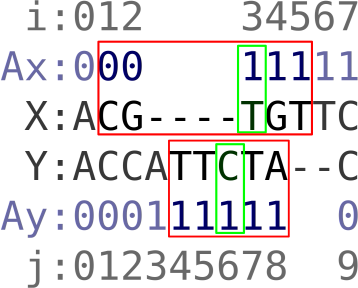
\includegraphics[width=\textwidth]{images/window_m}
                \caption{Match klasifikátor}
                \label{fig:window-m}
        \end{subfigure}%
        \qquad\qquad %add desired spacing between images, e. g. ~, \quad, \qquad etc.
          %(or a blank line to force the subfigure onto a new line)
        \begin{subfigure}[b]{0.35\textwidth}
                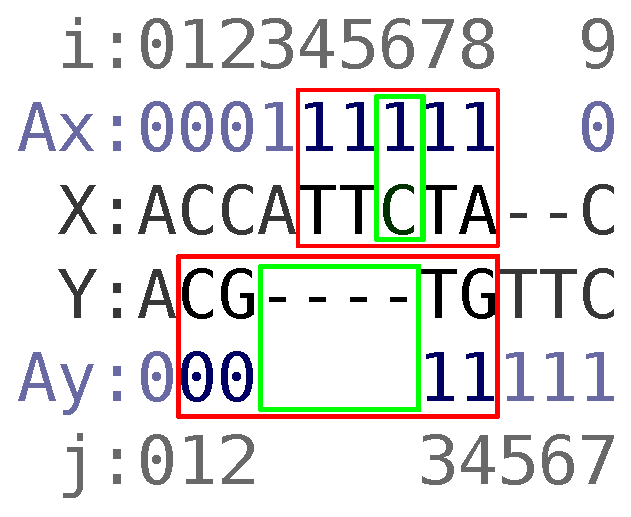
\includegraphics[width=\textwidth]{images/window_i}
                \caption{Indel klasifikátor}
                \label{fig:window-i}
        \end{subfigure}
        \caption[Okno klasifikátora]{Okno klasifikátora pre pozície $i = 6$ a $j = 3$}
\end{figure}

\subsubsection{Typ dát A~- okno bez úpravy}

Ako prvý typ dát sme zobrali okno tak, ako sme ho definovali v~predošlej sekcii. Dáta obsahujú priamo všetky bázy a anotácie tak, ako sú v~okne.

\subsubsection{Typ dát B - zhody v~stĺpcoch okna}

Druhý typ dát obsahuje aktuálnu bázu spolu s~jej anotáciami a navyše pole veľkosti $k*w$,
ktoré má na $i$-tom mieste jedna ak $okno_X[i] = okno_Y[i]$, ináč nula
($w$ je veľkosť okna, $k$ je veľkosť bloku, $okno_X$ je časť okna zodpovedajúca sekvencii $X$ a $okno_Y$ sekvencii $Y$).
V~Indel klasifikátore je jedna malá zmena: pozícia 0 aj 1 v~$x$-ovej sekvencii sú porovnávané s~pozíciou 1 v~$y$-ovej a pozícia 2 v~$x$-ovej sa porovnáva s~pozíciou 2 v~$y$-ovej.
Pozíciu 1 v~$y$-ovej sekvencii sme zopakovali preto, že sme experimentom zistili, že pre klasifikátor je dôležitá.

\subsubsection{Typ dát C - matica zhôd v~okne}

Tretí typ dát je podobný ako typ B. Rozdiel je v~tom, že teraz pole obsahuje nielen zhody po dvojiciach ale celú maticu zhôd. Teda opäť máme aktuálne bázy s~anotáciami a pole má veľkosť $k*w^2$. Každý riadok sa skladá z~jednotlivých blokov a v~tabuľke v~$x$-tom riadku, $y$-tom stĺpci a $i$-tom mieste v~bloku je jedna práve
vtedy, keď $okno_X[x+i] = okno_Y[y+i]$.

\subsubsection{Typ dát D - kombinácia A~a B}

Posledný typ dát je kombináciou typov dát A~a~B. Dáta opäť obsahujú všetky bázy a anotácie tak ako v~type A~a navyše sme pridali pole zhôd z~dát typu~B. Táto informácia je síce redundantná a klasifikátor by si ju mal vedieť odvodiť aj sám, no experimenty ukázali, že to pomôže.

\subsection{Trénovanie a testovanie klasifikátorov}
\label{subsec:clf-training}
Pre oba typy klasifikátorov sme sa snažili nájsť vhodné pozitívne a negatívne trénovacie príklady. Z~oboch sme do trénovacej množiny zahrnuli rovnako, aby bola trénovacia množina vyvážená. Ak by sme nemali vyváženú trénovaciu množinu, klasifikátory by zvýhodnili triedu, ktorej príkladov by bolo viacej. Napríklad, keby sme pri Indel klasifikátore zobrali všetky pozície s~medzerou ako pozitívne a všetky zarovnané pozície ako negatívne príklady, klasifikátor, ktorý by dával hodnotu nula, by mal pomerne vysokú úspešnosť, pretože zarovnaných pozícií je rádovo viac ako pozícií s~medzerou. Preto by natrénovaný klasifikátor mal tendenciu dávať nižšie hodnoty, aby znížil trénovaciu chybu a tomu sa chceme vyhnúť.

Výber pozitívnych príkladov bol v~oboch prípadoch intuitívny. Pri výbere negatívnych príkladov sme sa museli zamyslieť nad vhodným protipólom k~pozitívnym dátam.

\subsubsection{Výber pozitívnych a negatívnych príkladov pre Match klasifikátor}
% \label{subsec:matchtraining}

Match klasifikátor sme chceli natrénovať tak, aby pre pozície, ktoré majú byť pri sebe, dával hodnoty blízke jednej a pre pozície ktoré k~sebe byť zarovnané nemajú dával hodnoty blízke nule.
Ako pozitívne príklady sme teda vybrali pozície z~trénovacích sekvencií, ktoré boli zarovnané k~sebe.

Ako negatívne príklady sme vyskúšali dva prístupy: \textit{náhodné dáta} a \textit{dáta s~posunom}.

\paragraph{Náhodné dáta:} Náhodné dáta sme vyberali ako náhodné pozície, ktoré neboli zarovnané k~sebe. Toto sa však ukázalo ako nedostatočné riešenie.
% Ľahko sa totiž mohlo stať, že sme ako negatívny príklad vybrali
%  že sa mohlo ľahko stať, že sa k~sebe dostali pozície s~okolím, ktoré boli od seba pomerne ďaleko a tak sa mohlo ľahko stať, že v~inej sekvencii, by mohli byť zarovnané k~sebe.
Preto sme sa rozhodli pristúpiť k~inému spôsobu výberu negatívnych vzoriek.

\paragraph{Dáta s~posunom:} Dáta s~posunom sme vyberali posunutím jednej z~dvoch pozícií v~zarovnanom okne.
Počas zarovnávania sa totiž väčšinou lokálne rozhodujeme, či zarovnať dané pozície k~sebe, alebo vložiť medzeru. Ak by sme vložili medzeru, nastal by posun v~jednej zo sekvencií. Rozhodli sme sa teda týmto inšpirovať a vyrábať negatívne príklady posunom zarovnaných pozícií. Pre každú zarovnanú pozíciu si najskôr rovnomerne náhodne vyberieme sekvenciu, ktorú budeme posúvať a potom z~exponenciálneho rozdelenia náhodne vyberieme veľkosť posunu. Presný vzťah pre výpočet posunu $\Delta$ je
$$\Delta = \left(2D-1\right)\cdot \left(1+\lfloor S\rfloor\right)\qquad D\sim Alt(0.5),\, S\sim Exp(0.75),$$
kde prvý člen nám určuje smer posunu (čo je to isté ako: ktorá sekvencia sa bude posúvať) a druhý člen určuje veľkosť posunu (chceme celočíselnú hodnotu $\geq 1$).

\subsubsection{Výber pozitívnych a negatívnych príkladov pre Indel klasifikátor}

Indel klasifikátor sme chceli natrénovať tak, aby pre miesta, ktoré majú byť zarovnané s~medzerou, dával čo najvyššie hodnoty a pre miesta, ktoré nemajú byť zarovnané k~medzere, dával čo najnižšie hodnoty. Ako pozitívne príklady sme sa teda rozhodli vyberať pozície, ktoré boli v~trénovacích sekvenciách zarovnané k~medzere. Ako negatívne príklady sme vybrali pozície, ktoré boli zarovnané k~sebe, teda tie isté, čo sme pri trénovaní Match klasifikátora považovali za pozitívne. Akurát v~tomto prípade mala jedna zo sekvencií okno skrátené o~jedna, teda akoby bola medzera pred bázou, s~ktorou je aktuálne uvažovaná pozícia zarovnaná.

\subsubsection{Parametre trénovacej a testovacej množiny}
\label{subsec:clf-training-sets}
Dáta pre naše experimenty pochádzajú z~nášho simulátora. Trénovacia sada sa skladá z~20 zarovnaní sekvencií, pričom každé zarovnanie má dĺžku 10000. Celá trénovacia sada pre Match klasifikátor má 329428 príkladov. Pre Indel klasifikátor má sada 34150 príkladov.
Testovacia sada sa skladá z~jedného zarovnania s~dĺžkou 10000. Pre Match klasifikátor obsahuje 16498 príkladov. Pre Indel klasifikátor obsahuje 1674 príkladov.
Vo všetkých sadách je polovica príkladov pozitívnych a polovica negatívnych.

\section{Výsledky experimentov}

% - Stredobodom tejto podkapitoly by mala byt prehladna tabulka, ktora pre kazdu kombinaciu trenovacich dat (nahodne/diagonalne), atributov (A/B/C/D) uvedie a klasifikator (Match/Indel) uvedie: trenovaciu chybu, testovaciu chybu, najdolezitejsie atributy (bud prvych k najdolezitejsich alebo s dolezitostou vacsou ako nejake cislo), nedolezite atributy (atributy s dolezitostou mensou ako volaco?). Tato tabulka potom dava zaklad ku diskusiam.
% - Podkapitolu zacnes tym, ze povies - Pouzili sme klasifikatory tak, ako sme napisali v podkapitole 3.2 a vysledky su v tabulke.
% - Potom uz len popisujes ZAUJIMAVE ukazy z tabulky, pricom grafy a pod. uvadzas len pre tie priklady, kde potrebujes dalsiu evidenciu navyse oproti udajom, ktore uz su uvedene vo velkej tabulke. NEZAUJIMAVE ukazy (t.j. ak je vsetko tak, ako by clovek priamo ocakaval) popisovat netreba.
% - Asi sa chces venovat aj nejakym sposobom distribuciam skore, ale tam chces zasa len ukazat porovnanie najlepsieho a najhorsieho grafu. (Kedze toto je asi dolezite pre vyber "finalneho" klasifikatora, ktory pojde do HMM...)

Použili sme klasifikátory tak, ako sme popísali v~sekcii \ref{sec:use-rf-alignment} a výsledky sa nachádzajú v~tabuľke \ref{tab:clf-results}.

\begin{table}[htp]
\catcode`\-=12
\centering
\begin{subtable}{\textwidth}
\centering
\begin{tabular}{ccccc}
\toprule
\multirow{2}{*}{Typ dát} & \multicolumn{2}{c}{chyba} & \multicolumn{2}{c}{atribúty}\\
\cmidrule(r){2-3}\cmidrule{4-5}
 & trénovacia & testovacia & najvýznamnejšie & najbezvýznamnejšie\\
\midrule
A~& 93,07\% & 83,57\% & $x_0,\, y_{-1},\, y_{1},\, x_*,\, y_*$ & $\{a,b\}_*$\\
B & 84,05\% & 84.31\% & $m_{-1},\, m_0,\, m_*$ & $l_*$ \\
C & 80,44\% & 79,79\% & $m_{-2,-2},\, m_{2,2}, l_{-1,-1}, l_{1,1}, m_{0,0}$ & ostatné\\
D & 93,65\% & 84,32\% & $m_0, m_{-1}, m_1, m_2, m{-2}$ & $l_*,\, \{a,b\}_*$\\
\bottomrule
\end{tabular}
\caption{Match klasifikátor}
\end{subtable}

\vspace{1cm}

\begin{subtable}{\textwidth}
\centering
\begin{tabular}{ccccc}
\toprule
\multirow{2}{*}{Typ dát} & \multicolumn{2}{c}{chyba} & \multicolumn{2}{c}{atribúty}\\
\cmidrule(r){2-3}\cmidrule{4-5}
 & trénovacia & testovacia & najvýznamnejšie & najbezvýznamnejšie\\
\midrule
A~& 88,51\% & 74,13\% & $x_0,\, x_{1},\, x_{-1},\, x_*, y_*$ & $\{a,b\}_*$\\
B & 77,17\% & 75,75\% & $m_0,\, m_{-1},\, m_{-2}$ & $l_*,\, m_1,\, m_2$ \\
C & 78,03\% & 75,03\% & $l_{2,2},\,m_{-2,-2},\,m_{0,1},\,l_{-1,-1},\, x_0,\,a_0$ & ostatné\\
D & 88,78\% & 76,46\% & $m_0, m_{-1}, m_{-2}, x_1, \{x, y\}_*$ & $\{l,a,b\}_*$\\
\bottomrule
\end{tabular}
\caption{Indel klasifikátor}
\end{subtable}
\caption[Porovnanie vlastností klasifikátorov]{Porovnanie vlastností klasifikátorov pri rôznych typoch dát.}
\label{tab:clf-results}
\end{table}

\subsection{Dôležitosť atribútov}

Atribúty sme označili takto: stredná pozícia je 0, pozície naľavo sú -1, -2 a pozície napravo 1 a 2, pričom v~Indel klasifikátore v~sekvencii s~medzerou pozícia 0 chýba. Bázy v~sekvencii $X$ označujeme $x_i$ a v~$Y$ $y_i$. Anotácie v~sekvencii $X$ označujeme $a_i$ a v~$Y$ $b_i$. Zhody medzi bázami $i,\, j$ budeme označovať $m_{i, j}$, pričom označenie zhôd v~type dát B a D zjednodušíme na $m_i$. Podobne zhody medzi anotáciami označíme $l_{i, j}$ (resp. $l_i$).

V~tabuľke \ref{tab:clf-results} si môžeme všimnúť, že klasifikátory sa zamerali najmä na bázy a okrem prípadu C anotácie skoro nebrali do úvahy.
Toto správanie zodpovedá tomu, že v~praxi bázy majú podstatne väčší význam pri zarovnávaní sekvencií.

V~prípade dát typu A~a B sa Match klasifikátory nezamerali na stredné bázy ako by sme to čakali, ale všetky bázy brali približne s~rovnakou váhou. Indel klasifikátory na tom boli podobne, hoci v~prípade dát typu B je vidieť výraznejšiu preferenciu atribútu zhody báz $x_0, y_1$ ($l_0$), avšak atribúty $l_1$ a $l_2$ klasifikátoru neprišli dôležité.

Pri type dát C si môžeme všimnúť, že najdôležitejšie atribúty sú na uhlopriečke, čo zodpovedá typu dát B, ibaže v~tomto prípade sa nám vyskytli na niektorých pozíciách anotácie namiesto báz.
Avšak ak sa nám tam vyskytla anotácia, bázu už klasifikátor nepovažoval za dôležitú a aj naopak.
Indel klasifikátor navyše považoval za dôležitejšiu aj bázu na aktuálnej pozícii a jej anotáciu. Pri type dát C, na rozdiel od ostatných, klasifikátor viac berie do úvahy aj anotácie.


\begin{figure}[htbp]
        \centering
        \begin{subfigure}[t]{0.4\textwidth}
                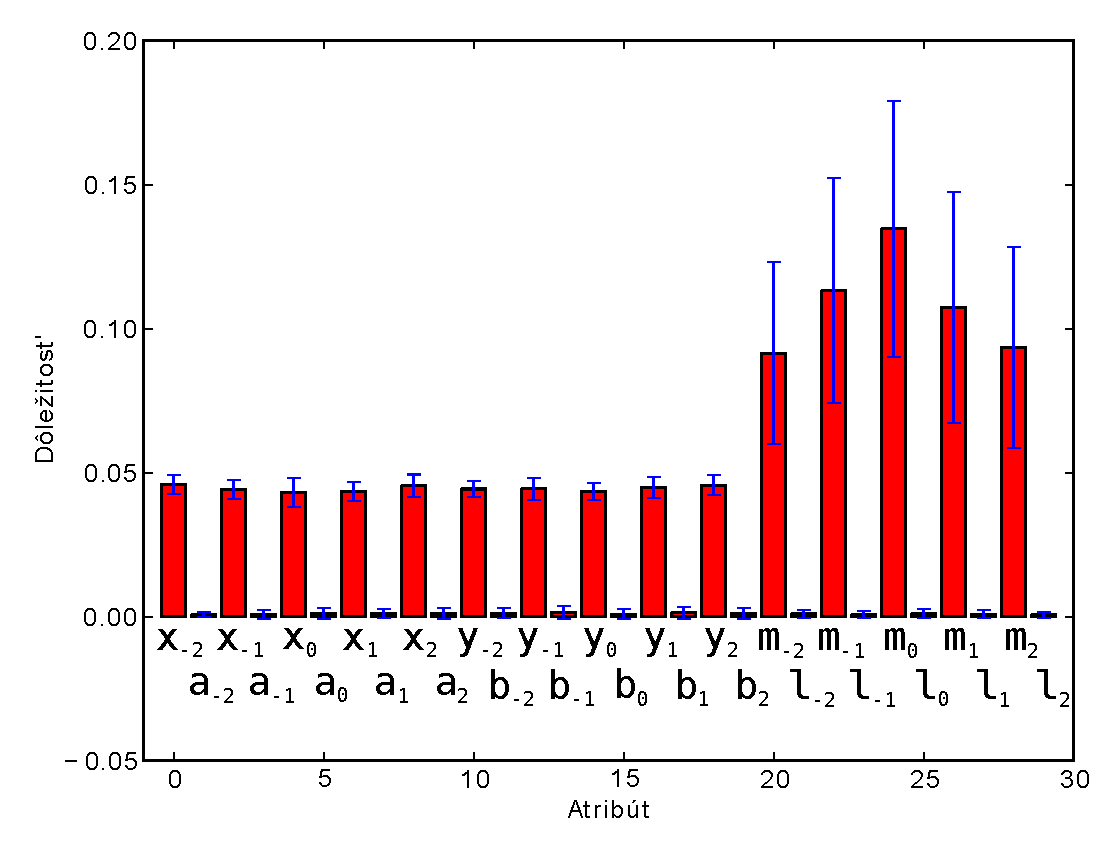
\includegraphics[width=\textwidth]{images/clf_fi/randomforest_combined_5_bars}
                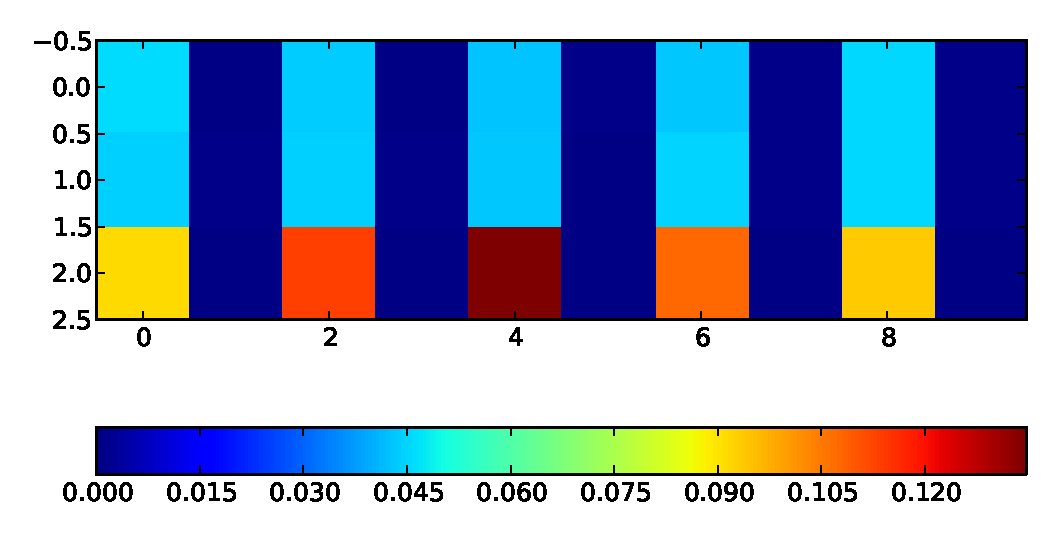
\includegraphics[width=\textwidth]{images/clf_fi/randomforest_combined_5_heatmap}
                \caption{Match klasifikátor}
                \label{fig:datatype4-m}
        \end{subfigure}%
        \qquad\qquad %add desired spacing between images, e. g. ~, \quad, \qquad etc.
          %(or a blank line to force the subfigure onto a new line)
        \begin{subfigure}[t]{0.4\textwidth}
                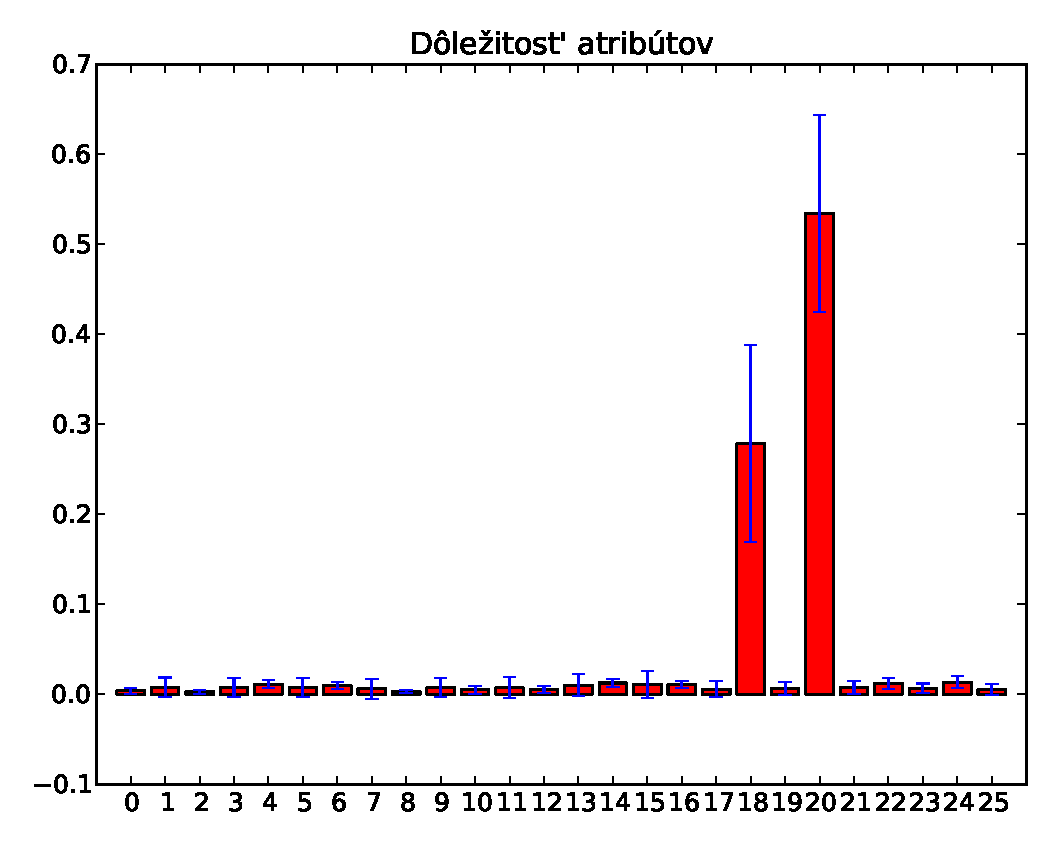
\includegraphics[width=\textwidth]{images/clf_fi/randomforest_combined_5_indel_bars}
                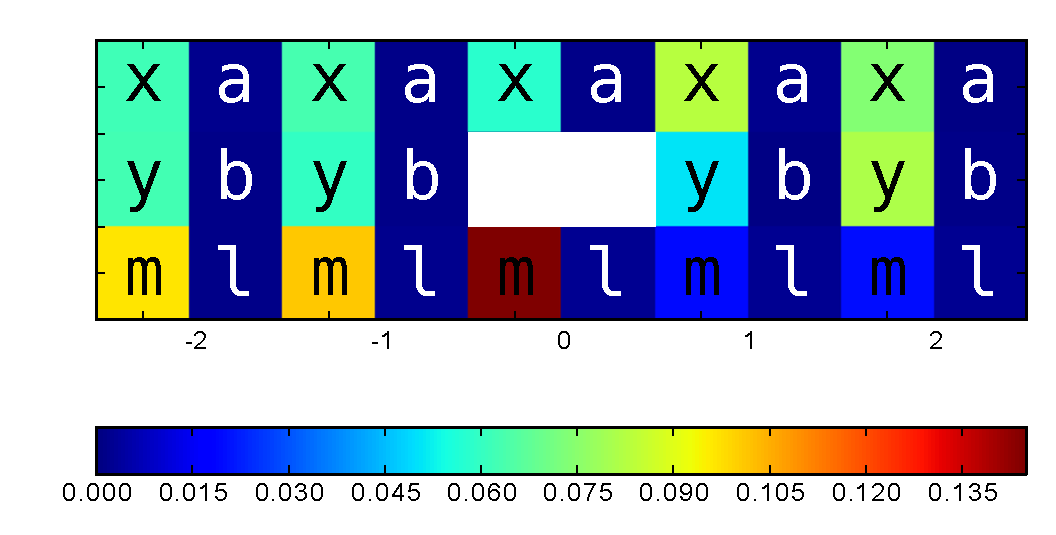
\includegraphics[width=\textwidth]{images/clf_fi/randomforest_combined_5_indel_heatmap}
                \caption{Indel klasifikátor}
                \label{fig:datatype4-i}
        \end{subfigure}
        \caption[Dôležitosť atribútov pre typ dát D]{
        \textbf{Dôležitosť atribútov pre typ dát D} - hodnoty sú normalizované, aby súčet bol jedna, modrý pásik označuje štandardnú odchýlku cez jednotlivé stromy v~náhodnom lese.
        Pod grafom je tepelná mapa pre lepšiu vizualizáciu.}
        \label{fig:datatype4}
\end{figure}


Pri dátach typu D sme dostali v~prípade Match klasifikátora očakávanú distribúciu dôležitosti atribútov (obr. \ref{fig:datatype4}). Dáta typu B boli uprednostnené voči typu~A, avšak aj bázy z~typu A~boli dôležité. Pri Indel klasifikátore sme dostali graf, ktorý je zložením grafov z~dát typu A~a~B. Zaujímavosťou je, že pri tomto type dát má výraznejšiu úlohu práve zhoda na stredovej pozícii, teda pozície už nie sú také rovnocenné ako to bolo v~type~B.

\FloatBarrier

\subsection{Úspešnosť klasifikátora}

V~tabuľke \ref{tab:clf-results} vidíme, že hoci typ C obsahuje nadmnožinu atribútov B, jeho úspešnosť je nižšia a tento typ nemá zmysel používať. Ďalej si môžeme všimnúť, že kombinácia typov A~a B využila klady oboch a mierne ich vylepšila.

\begin{figure}[htbp]
        \centering
        \begin{subfigure}[t]{0.4\textwidth}
                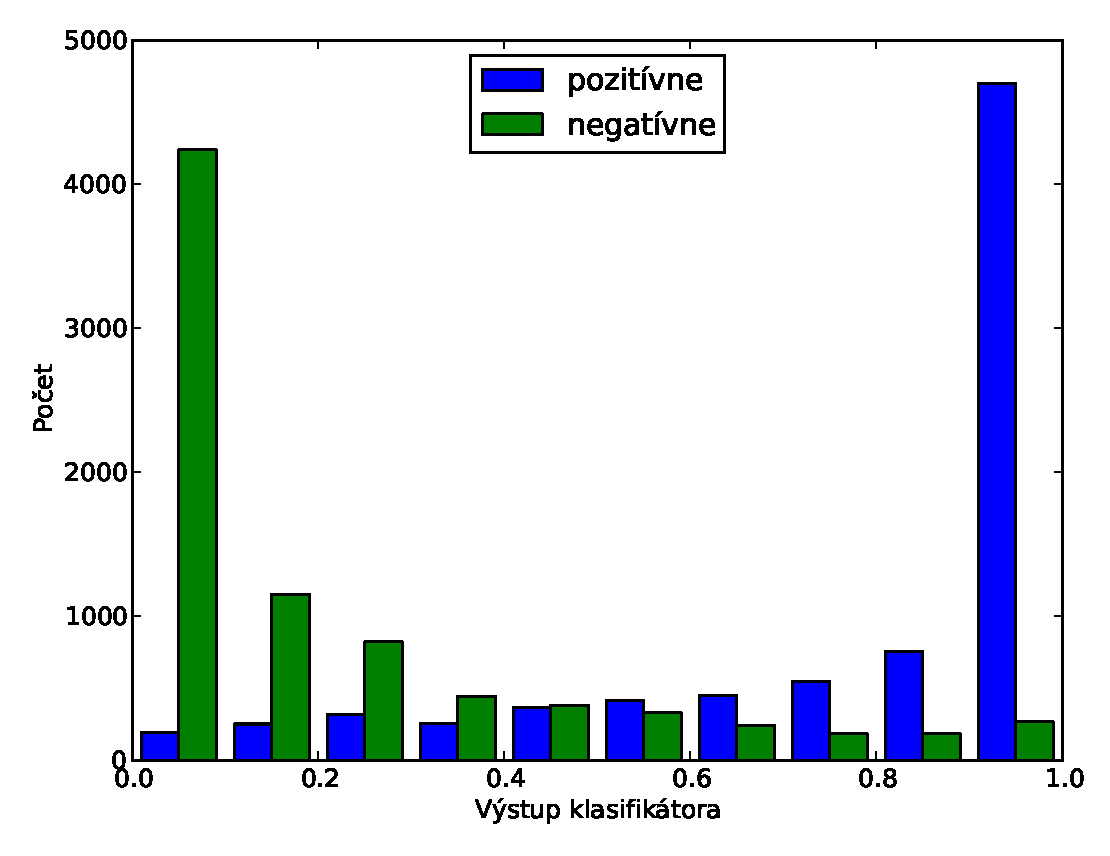
\includegraphics[width=\textwidth]{images/clf_fi/randomforest_combined_5_test}
                \caption{Match klasifikátor}
                \label{fig:datatype4-out-m}
        \end{subfigure}%
        \qquad\qquad %add desired spacing between images, e. g. ~, \quad, \qquad etc.
          %(or a blank line to force the subfigure onto a new line)
        \begin{subfigure}[t]{0.4\textwidth}
                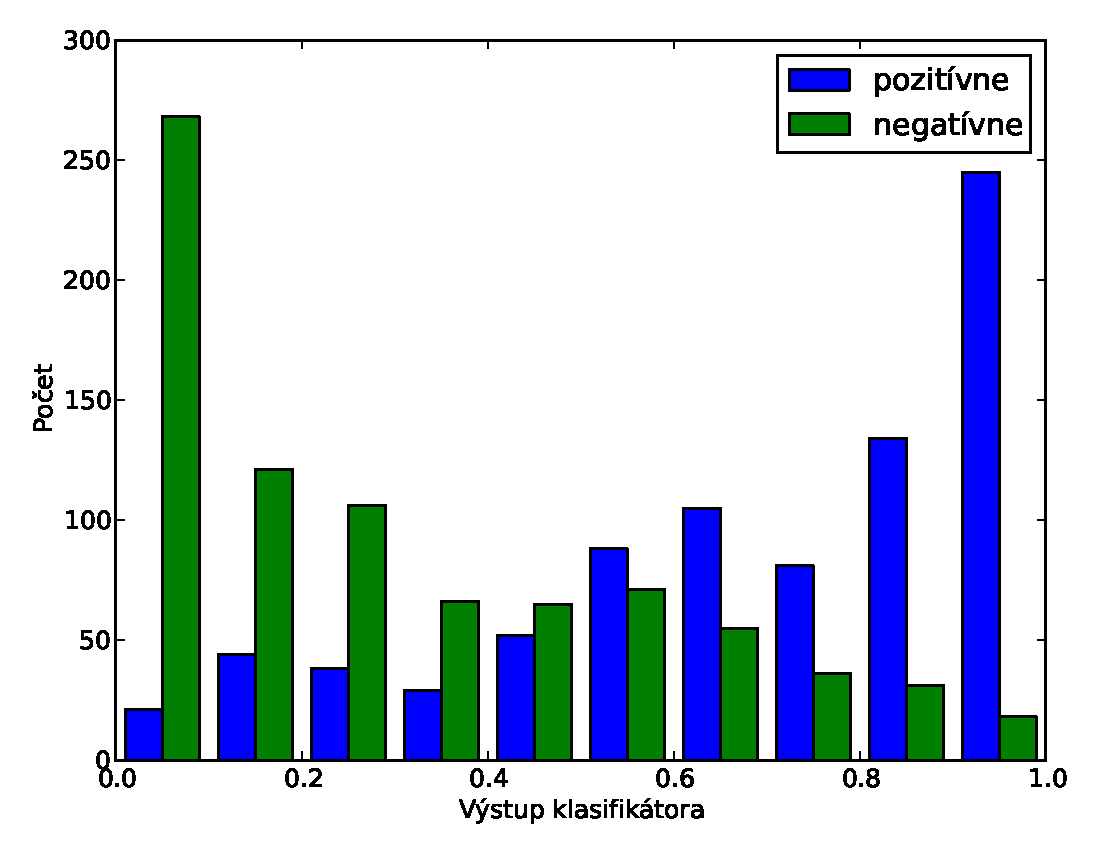
\includegraphics[width=\textwidth]{images/clf_fi/randomforest_combined_5_indel_test}
                \caption{Indel klasifikátor}
                \label{fig:datatype4-out-i}
        \end{subfigure}
        \caption[Distribúcia výstupu z~klasifikátora pri type D]{Distribúcia výstupu z~klasifikátora pri type dát D -- modré sú pozitívne príklady a zelené su negatívne. Na $x$-ovej osi je výstup klasifikátora a na $y$-je počet inštancií, pre ktoré výstup z~klasifikátora padol do daného chlievika}
        \label{fig:datatype4-out}
\end{figure}

Úspešnosť klasifikátorov s~rôznym typom dát sme skúmali aj podrobnejšie, pozerali sme sa aj na distribúciu výstupov klasifikátora. Silný klasifikátor má totiž distribúciu takú, že väčšina pozitívnych príkladov má vysoké výstupné hodnoty a väčšina negatívnych klasifikátorov má nízke výstupné hodnoty. Najlepšiu distribúciu výstupov sa nám podarilo dosiahnuť práve pri type D (obr. \ref{fig:datatype4-out}). Na obrázku \ref{fig:datatype-bad-out} sú pre porovnanie najhoršie distribúcie z~ostatných typov dát.
\begin{figure}[htbp]
        \centering
        \begin{subfigure}[t]{0.4\textwidth}
                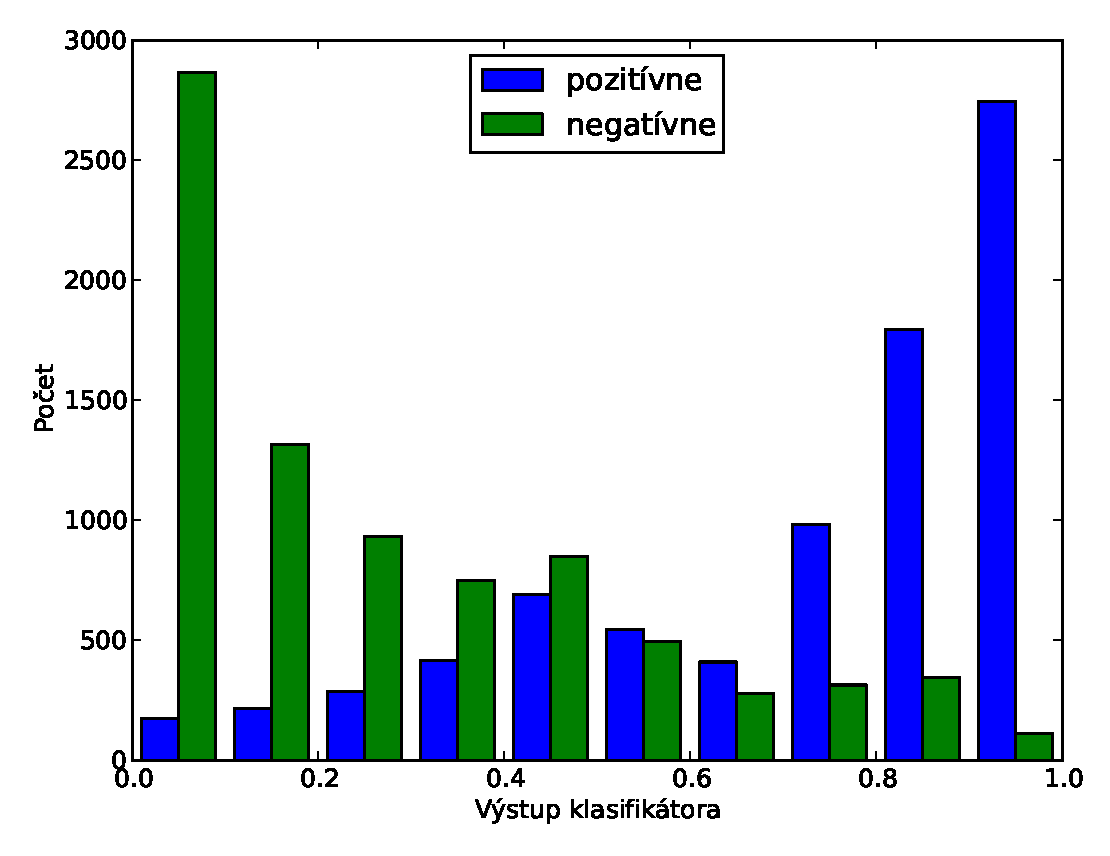
\includegraphics[width=\textwidth]{images/clf_fi/randomforest_fullcmp_5_test}
                \caption{Typ C: Match klasifikátor}
                \label{fig:datatype1-out-m}
        \end{subfigure}%
        \qquad\qquad %add desired spacing between images, e. g. ~, \quad, \qquad etc.
          %(or a blank line to force the subfigure onto a new line)
        \begin{subfigure}[t]{0.4\textwidth}
                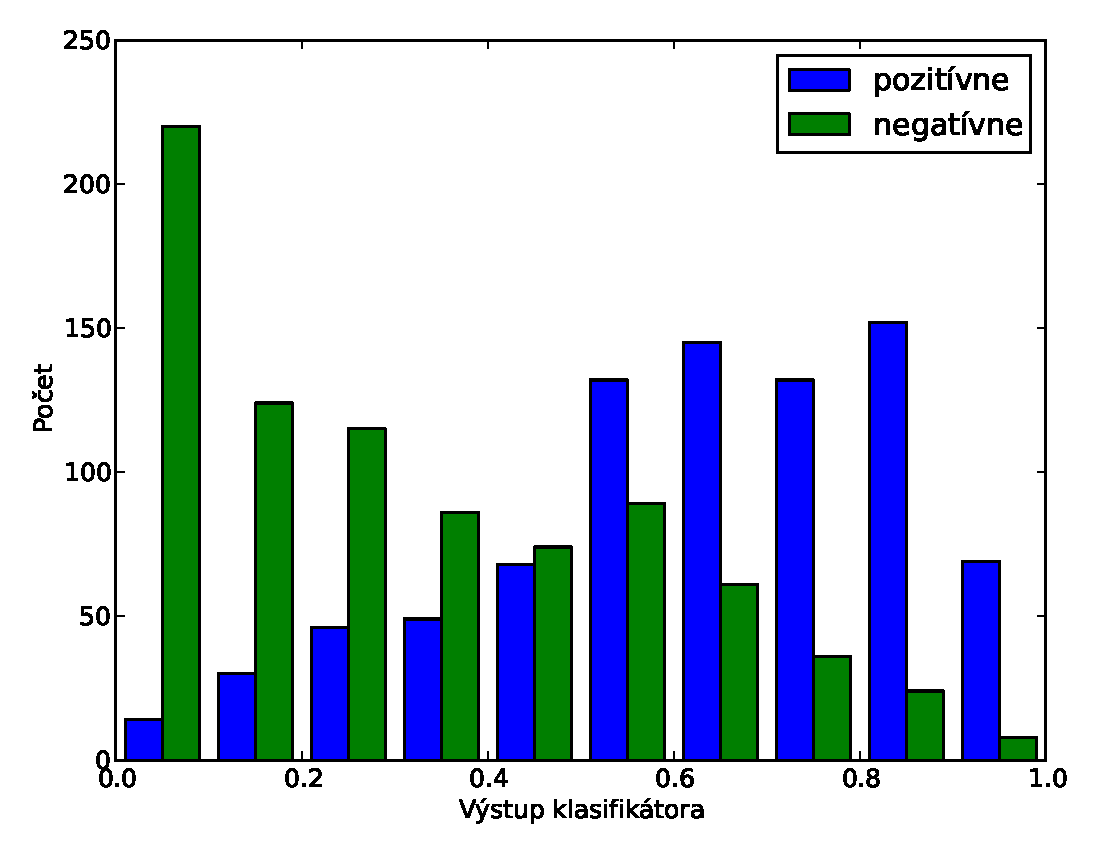
\includegraphics[width=\textwidth]{images/clf_fi/randomforest5_indel_test}
                \caption{Typ A: Indel klasifikátor}
                \label{fig:datatype1-out-i}
        \end{subfigure}
        \caption[Horšie distribúcie výstupov z~klasifikátora]{Horšie distribúcie výstupov z~klasifikátora -- modré sú pozitívne príklady a zelené sú negatívne. Na $x$-ovej osi je výstup klasifikátora a na $y$-je počet inštancií, pre ktoré výstup z~klasifikátora padol do daného chlievika}
        \label{fig:datatype-bad-out}
\end{figure}

\FloatBarrier
\section{Zhrnutie}

V~tejto kapitole sme si predstavili klasifikátory, ktoré použijeme v~našich modeloch. Uviedli sme dva typy klasifikátorov -- pre Match stav a Inzert stav. Venovali sme sa výberu atribútov pre klasifikátory a ich trénovaniu. Predstavili sme si štyri množiny atribútov pre naše klasifikátory, pre ktoré sme porovnali vlastnosti klasifikátora.

Nakoniec sme sa rozhodli použiť ako množinu atribútov typ D, pretože s~týmito atribútmi mali klasifikátory najlepšie vlastnosti a aj najvyššiu úspešnosť.
